\documentclass[10pt,a4paper]{article}
\usepackage[T1]{fontenc}
\usepackage[utf8]{inputenc}
\usepackage[czech]{babel}
\usepackage{lmodern}         % <- Přidáno pro opravu chyby fontu
\usepackage{csquotes}
\usepackage{xcolor}
\usepackage{geometry}
\usepackage{microtype}
\usepackage{graphicx}
\usepackage{booktabs}
\usepackage{setspace}
\usepackage{hyperref}
\geometry{left=2.5cm, right=2cm, top=2.5cm, bottom=3cm}

\title{\Huge{Zpráva k projektu INC}}
\author{Radim Pokorný \\ Login: xpokorr00}
\date{\today}

\begin{document}

\maketitle

\section{Návrh obvodu}
\begin{center}
    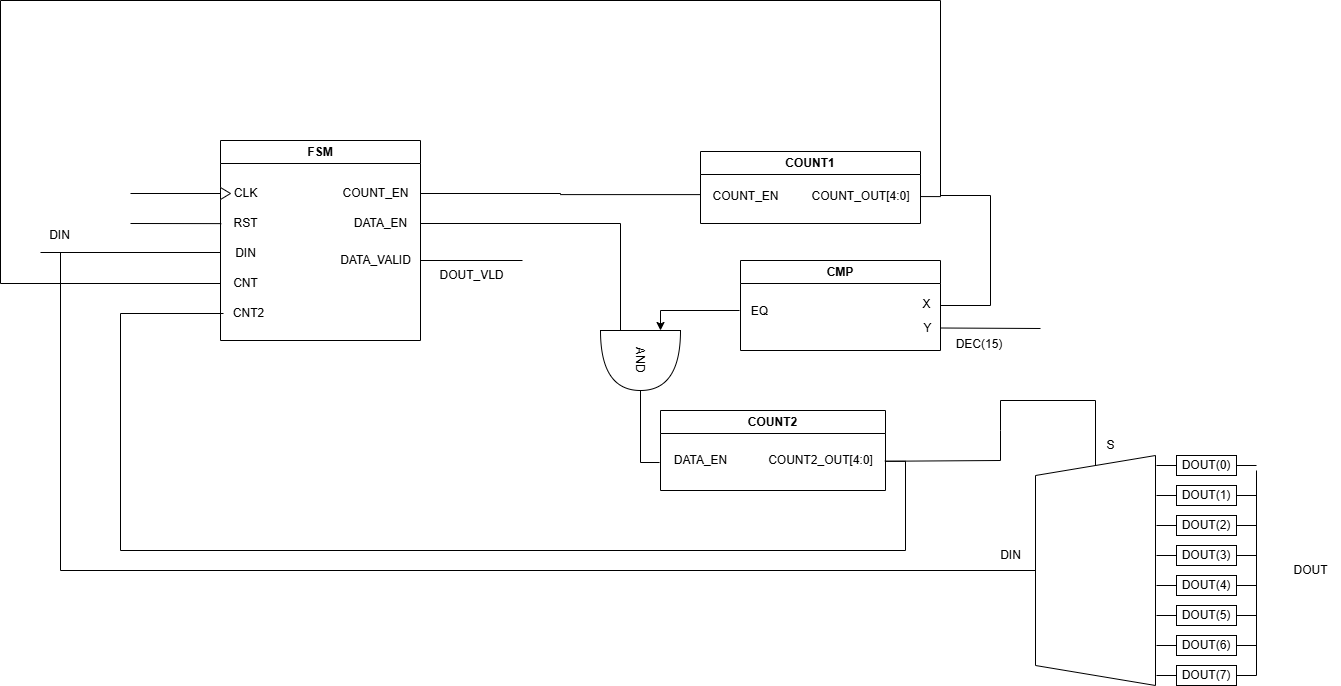
\includegraphics[width=0.9\textwidth]{navrh_obvodu.png}
\end{center}

\subsection{Popis součástek}

\begin{itemize}
    \item \textbf{FSM} -- Automat pro příjem dat.
    \item \textbf{COUNT1} -- Čítač hodinového signálu s max. délkou 5 bitů
    \item \textbf{COUNT2} -- Čítač dat (bitů) s max. délkou 4 bitů
    \item \textbf{DEMULTIPLEXOR} -- Spojení dát do jednoho výstupu
\end{itemize}

\subsection{Popis činnosti}
Do automatu FSM se zasílají 3 signály CLOCK, RESET a DATA\_INPUT. První výstup s kterým se pracuje, je COUNT\_EN, který
povoluje čítači COUNT1 počítat. Jakmile se dostane do 16. cyklu, tak nabije logickou "1" pomocí funkce CMP s dvěma vstupy DEC(15) a COUNT\_OUT.
Výsledek se dostane do logické funkce AND a obvod zajimá, jestli je aktivní 2. výstup FSM DATA\_EN. Jestliže ano, do funkce AND přichází 
2 logické "1", tak logický výstup AND je "1". Tím pádem se aktivuje vstup v DATA\_EN v součástce COUNT2, která zasílá signál hodnoty data do multiplexoru
a společně s COUNT1 zasílá své výstupy zpět do FSM automatu, aby mohl dál správně fungovat. Jako druhý vstup multiplexoru je DIN, který je propojen s vstupem
automatu. Ve finální fázi se v multiplexoru shromáždí data a vytvoří se 1 výstup DOUT o délce 8 bitů.

\section{Diagram automatu}
\begin{center}
    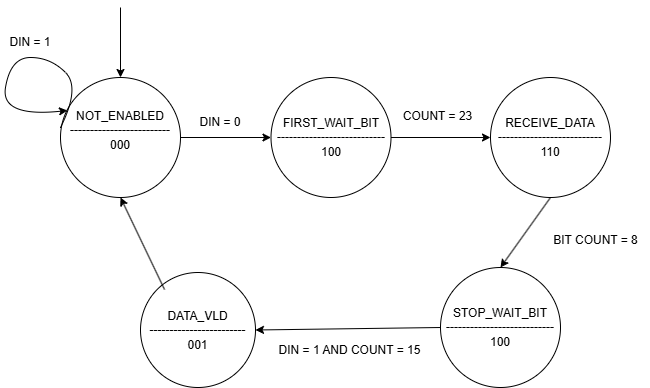
\includegraphics[width=0.9\textwidth]{automat.png}
\end{center}

\subsection{Stavy automatu}
Automat je navržen jako konečný stavový automat (FSM) pro příjem dat přes UART. Pracuje v pěti stavech:

\begin{itemize}
    \item \textbf{NOT\_ENABLED} -- Automat je neaktivní, čeká na start bit.
    \item \textbf{FIRST\_WAIT\_BIT} -- Čekání na ustálení start bitu.
    \item \textbf{RECEIVE\_DATA} -- Přijímání 8bitových dat.
    \item \textbf{STOP\_WAIT\_BIT} -- Čekání na stop bit.
    \item \textbf{DATA\_VLD} -- Data byla přijata a ověřena.
\end{itemize}

\noindent
Přechody mezi stavy jsou řízeny vstupními signály Data Input \texttt{(DIN)}, Clock Count \texttt{(CNT)} a Bit Count\texttt{(CNT2)}.

\subsection{Výstupy automatu (Moorův typ)}
Automat je typu \textbf{Moore}, protože výstupy závisí pouze na aktuálním stavu (a ne na vstupech).

Výstupní signály:

\begin{itemize}
    \item \textbf{COUNT\_EN} -- Aktivní ve stavech \texttt{FIRST\_WAIT\_BIT}, \texttt{RECEIVE\_DATA} a \texttt{STOP\_WAIT\_BIT}.
    \item \textbf{DATA\_EN} -- Aktivní pouze ve stavu \texttt{RECEIVE\_DATA}.
    \item \textbf{DATA\_VALID} -- Aktivní pouze ve stavu \texttt{DATA\_VLD}.
\end{itemize}

\subsection{Popis automatu}
Tento automat pracuje s 5 stavy, kde začíná na NOT\_ENABLED, zde čeká na logickou nulu, poté
dojde do stavu, kde čeká na FIRST\_BIT, v tomto stavu díky čítači COUNT setrvá 23 cyklů a poté přejde
do stavu RECEIVE\_DATA, kde dojde k přečtení 8 bitů. Poté čeká na STOP\_BIT, jakmile dostane logickou 1 a zároveň
čítač je v 15 cyklu, tak se přejde na poslední stav DATA\_VLD, kde proběhne podle názvu validace dat a
přechází se následně zpět do výchozího stavu NOT\_ENABLED.

\section{Ukázka simulace}
\begin{center}
    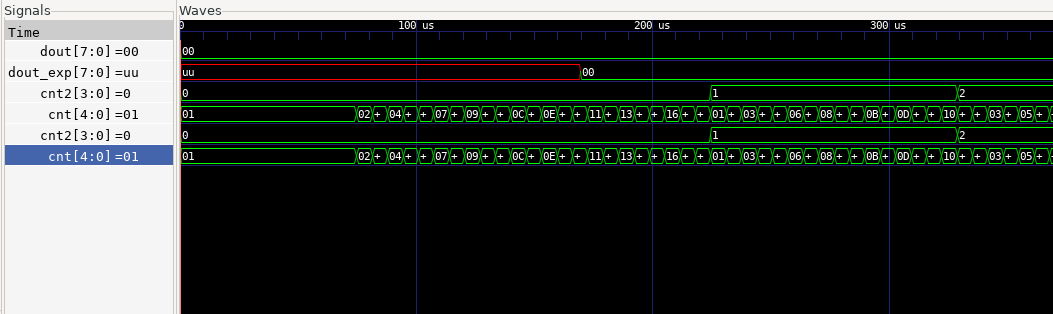
\includegraphics[width=0.9\textwidth]{gtkwave.png}
\end{center}

\end{document}